% Figure 4: Energy Extraction Schematic
% Author: Dr. Computernonymouse
% Description: System-level block diagram showing ZPE extraction architecture
%              with efficiency factors and cryogenic cooling system

\documentclass[tikz,border=10pt]{standalone}
\usepackage{tikz}
\usepackage{pgfplots}
\usepackage{amsmath}
\usepackage{amssymb}
\usepackage{siunitx}

\pgfplotsset{compat=1.18}
\usetikzlibrary{calc,arrows.meta,patterns,backgrounds,positioning,shapes.geometric,decorations.pathmorphing,shadows}

% Define system colors
\definecolor{blockblue}{RGB}{68,114,196}
\definecolor{blockgreen}{RGB}{112,173,71}
\definecolor{blockorange}{RGB}{237,125,49}
\definecolor{blockred}{RGB}{192,0,0}
\definecolor{cryoblue}{RGB}{142,180,227}
\definecolor{vacuumgray}{RGB}{128,128,128}
\definecolor{flowArrow}{RGB}{255,192,0}
\definecolor{coolingblue}{RGB}{91,155,213}

% Custom block style
\tikzstyle{mainblock} = [
    rectangle,
    rounded corners=3mm,
    minimum width=3cm,
    minimum height=1.5cm,
    text centered,
    draw=black,
    line width=1pt,
    font=\bfseries,
    drop shadow
]

\tikzstyle{efficiency} = [
    rectangle,
    rounded corners=1mm,
    minimum width=1.5cm,
    minimum height=0.6cm,
    text centered,
    draw=black,
    line width=0.5pt,
    font=\small
]

\tikzstyle{flowarrow} = [
    ->,
    >=Stealth,
    line width=3pt,
    flowArrow,
    shorten >=2mm,
    shorten <=2mm
]

\tikzstyle{coolingarrow} = [
    <->,
    >=Stealth,
    line width=1.5pt,
    coolingblue,
    dashed
]

\begin{document}

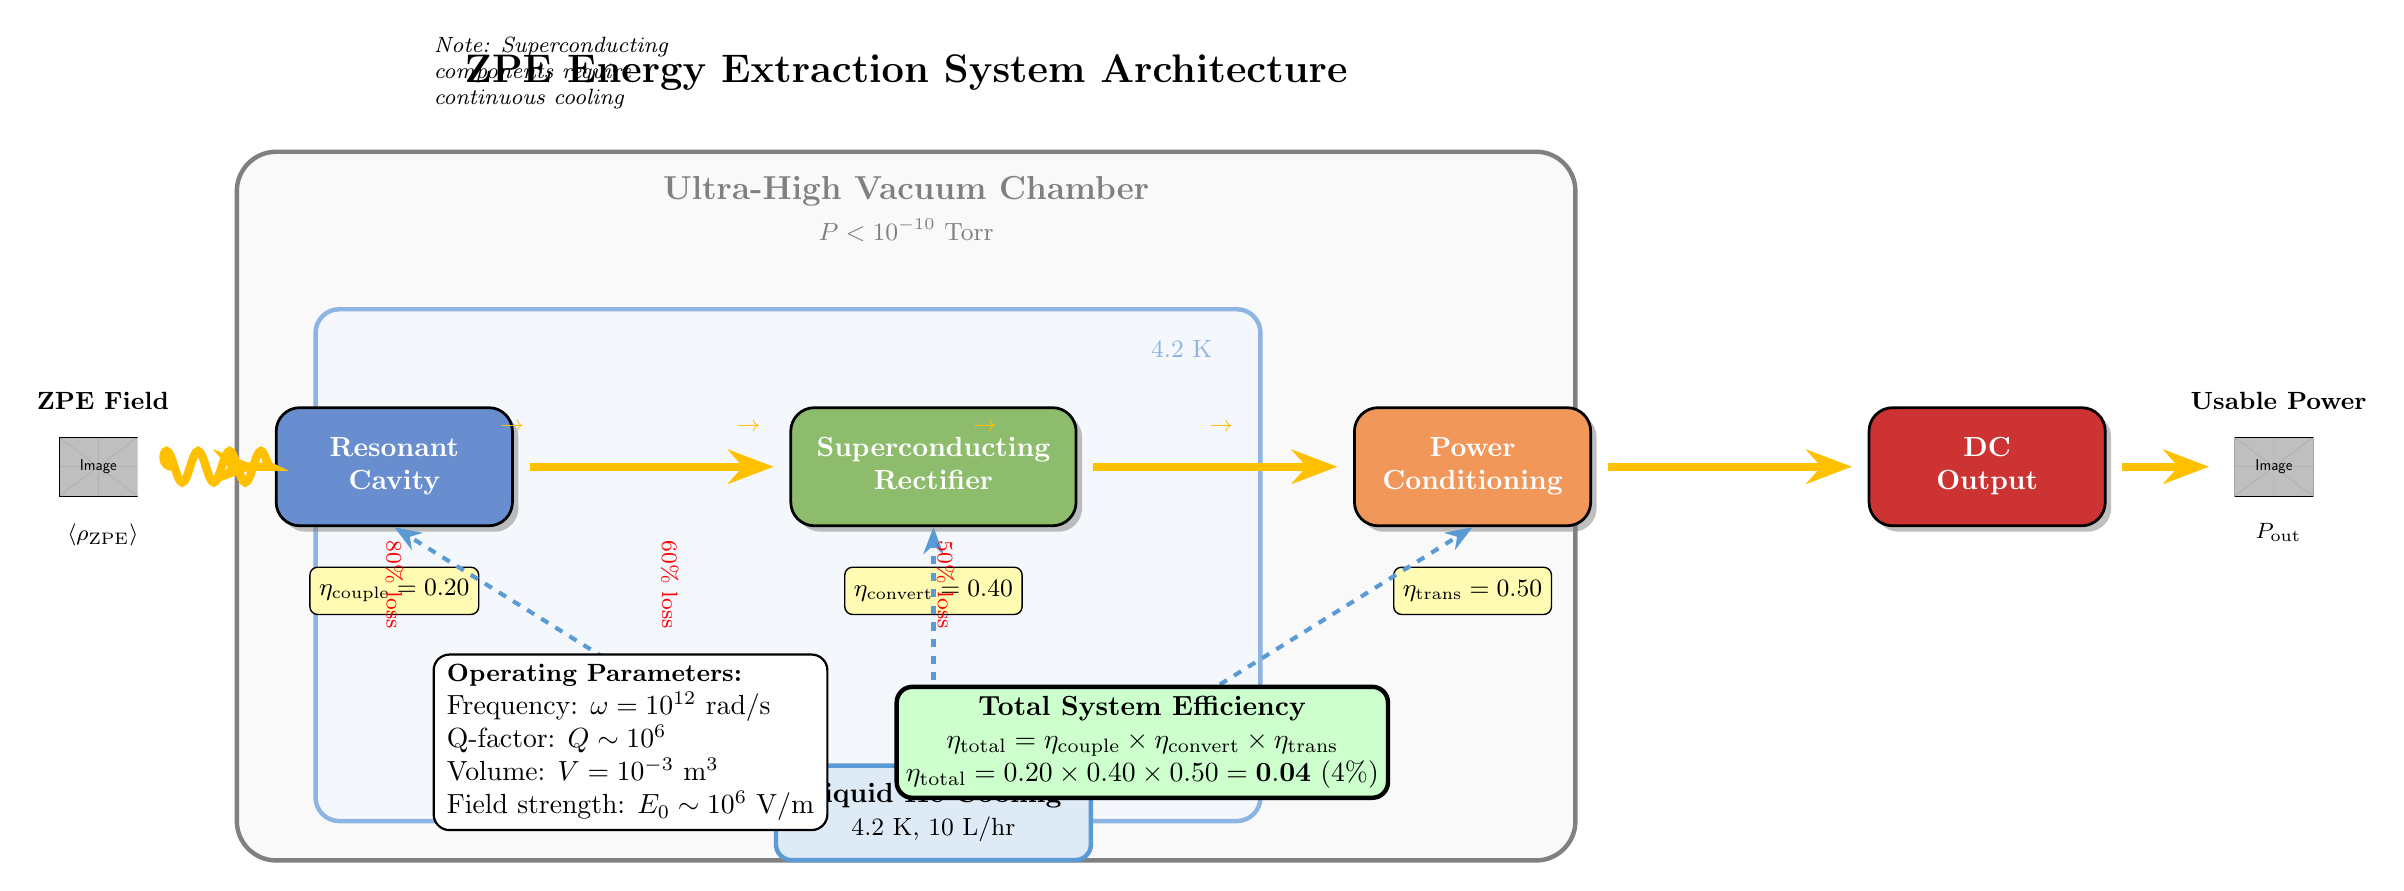
\begin{tikzpicture}[node distance=3.5cm]

% Background layers
\begin{scope}[on background layer]
    % UHV chamber boundary
    \draw[vacuumgray,ultra thick,rounded corners=5mm,fill=vacuumgray!5]
        (-2,-5) rectangle (15,4);
    \node[vacuumgray,font=\large\bfseries] at (6.5,3.5) {Ultra-High Vacuum Chamber};
    \node[vacuumgray,font=\small] at (6.5,3) {$P < 10^{-10}$ Torr};

    % Cryogenic region
    \draw[cryoblue,ultra thick,rounded corners=3mm,fill=cryoblue!10]
        (-1,-4.5) rectangle (11,2);
    \node[cryoblue,font=\small] at (10,1.5) {4.2 K};
\end{scope}

% Main system blocks
\node[mainblock,fill=blockblue!80,text=white] (cavity) at (0,0) {
    \begin{tabular}{c}
        Resonant\\Cavity
    \end{tabular}
};

\node[mainblock,fill=blockgreen!80,text=white,right=of cavity] (rectifier) {
    \begin{tabular}{c}
        Superconducting\\Rectifier
    \end{tabular}
};

\node[mainblock,fill=blockorange!80,text=white,right=of rectifier] (conditioning) {
    \begin{tabular}{c}
        Power\\Conditioning
    \end{tabular}
};

\node[mainblock,fill=blockred!80,text=white,right=of conditioning] (output) {
    \begin{tabular}{c}
        DC\\Output
    \end{tabular}
};

% Efficiency labels
\node[efficiency,fill=yellow!30,below=0.5cm of cavity] (eff1) {
    $\eta_{\text{couple}} = 0.20$
};

\node[efficiency,fill=yellow!30,below=0.5cm of rectifier] (eff2) {
    $\eta_{\text{convert}} = 0.40$
};

\node[efficiency,fill=yellow!30,below=0.5cm of conditioning] (eff3) {
    $\eta_{\text{trans}} = 0.50$
};

% Energy flow arrows
\draw[flowarrow] (cavity) -- (rectifier);
\draw[flowarrow] (rectifier) -- (conditioning);
\draw[flowarrow] (conditioning) -- (output);

% Input ZPE field
\node[left=1.5cm of cavity,align=center] (zpe) {
    \includegraphics[width=1cm]{example-image}
};
\node[above=0.1cm of zpe,font=\small\bfseries] {ZPE Field};
\node[below=0.1cm of zpe,font=\footnotesize] {$\langle\rho_{\text{ZPE}}\rangle$};

\draw[flowarrow,decorate,decoration={snake,amplitude=2mm,segment length=4mm}]
    (zpe) -- (cavity);

% Output power
\node[right=1.5cm of output,align=center] (power) {
    \includegraphics[width=1cm]{example-image}
};
\node[above=0.1cm of power,font=\small\bfseries] {Usable Power};
\node[below=0.1cm of power,font=\footnotesize] {$P_{\text{out}}$};

\draw[flowarrow] (output) -- (power);

% Cryogenic cooling system
\node[below=3cm of rectifier,align=center,draw=coolingblue,ultra thick,
      rounded corners=2mm,fill=coolingblue!20,minimum width=4cm,minimum height=1.2cm] (cryo) {
    \textbf{Liquid He Cooling}\\
    \small 4.2 K, 10 L/hr
};

% Cooling connections
\draw[coolingarrow] (cryo.north west) -- (cavity.south);
\draw[coolingarrow] (cryo.north) -- (rectifier.south);
\draw[coolingarrow] (cryo.north east) -- (conditioning.south);

% System parameters box
\node[draw=black,thick,rounded corners=2mm,fill=white!90,
      minimum width=5cm,align=left] at (3,-3.5) {
    \small
    \textbf{Operating Parameters:}\\
    Frequency: $\omega = 10^{12}$ rad/s\\
    Q-factor: $Q \sim 10^6$\\
    Volume: $V = 10^{-3}$ m$^3$\\
    Field strength: $E_0 \sim 10^6$ V/m
};

% Total efficiency calculation
\node[draw=black,ultra thick,rounded corners=2mm,fill=green!20,
      minimum width=6cm,align=center] at (9.5,-3.5) {
    \textbf{Total System Efficiency}\\
    $\eta_{\text{total}} = \eta_{\text{couple}} \times \eta_{\text{convert}} \times \eta_{\text{trans}}$\\
    $\eta_{\text{total}} = 0.20 \times 0.40 \times 0.50 = \mathbf{0.04}$ (4\%)
};

% Power flow indicators
\foreach \x in {1.5,4.5,7.5,10.5} {
    \node[font=\footnotesize,flowArrow] at (\x,0.5) {$\rightarrow$};
}

% Loss indicators
\node[font=\footnotesize,red,rotate=-90] at (0,-1.5) {80\% loss};
\node[font=\footnotesize,red,rotate=-90] at (3.5,-1.5) {60\% loss};
\node[font=\footnotesize,red,rotate=-90] at (7,-1.5) {50\% loss};

% Title
\node[font=\Large\bfseries] at (6.5,5) {ZPE Energy Extraction System Architecture};

% Technical notes
\node[font=\footnotesize,align=left] at (2,5) {
    \textit{Note: Superconducting}\\
    \textit{components require}\\
    \textit{continuous cooling}
};

\end{tikzpicture}

\end{document}